\documentclass[10pt]{beamer}
\usepackage{alltt}
\usepackage{graphicx}
\usepackage{xspace}
\usepackage{color}
\usepackage{amsmath}
\definecolor{linkcolor}{RGB}{16,65,69}

\newcommand{\ttt}[1]{\texttt{#1}}
\newcommand{\projname}{\ttt{bt}\xspace}

\newenvironment{monospace}{\begin{quote}\begin{alltt}}{\end{alltt}\end{quote}}

\author{Joe Colosimo \\ \small{colosimo@mit.edu} \\ Group 6}
\date{\today}


\usepackage{xmpmulti}
\usetheme{default}
\beamertemplatesolidbackgroundcolor{black}
\setbeamercolor{normal text}{fg=white}
\setbeamercolor{title}{fg=white}
\usecolortheme[named=white]{structure}
\setbeamertemplate{frametitle}[default][center]
\setbeamertemplate{navigation symbols}{}

\title{\projname}
\subtitle{A Hardware Beat Tracker}
\author{Joseph Colosimo}
\date{May 15, 2013}
\institute{Massachusetts Institute of Technology}


\begin{document}
\begin{frame}
    \titlepage
\end{frame}

\begin{frame}{Architecture}
    \begin{center}
        \includegraphics{fig/architecture.pdf}
    \end{center}
\end{frame}

\begin{frame}{Implementation}
    \begin{center}
        \includegraphics{fig/hwarch.pdf}
    \end{center}
\end{frame}

\begin{frame}{In Real Life}
    \begin{center}
        \includegraphics<1>[scale=0.45]{fig/dcbiasbrd.jpg}
        \includegraphics<2>[scale=0.5]{fig/setup.jpg}
    \end{center}
\end{frame}


\end{document}
